\documentclass{article}

\usepackage{fullpage}
\usepackage{graphicx}
\usepackage{color}
\usepackage{fancyhdr}
\usepackage{url}
\usepackage{subfig}
\usepackage{multirow}
\usepackage[table]{xcolor}
\usepackage{amsmath,bm}
\usepackage{amssymb}
\usepackage{amsthm}
\usepackage{amsfonts}
\usepackage[round]{natbib}
\usepackage{enumitem,xcolor}
\usepackage[multiple]{footmisc}

\usepackage[
 pdftitle={Capstone Report - Udacity Machine Learning Nanodegree},
 pdfsubject={Machine Learning, Reinforcement Learning, Deep Learning, Artificial Intelligence, Games},
 pdfauthor={David Robles},
 pdfpagemode=UseOutlines,
 pdfborder= {0 0 1.0},
 bookmarks,
 bookmarksopen,
 colorlinks=true,
 citecolor=blue,
 linkcolor=blue, %
 linkbordercolor=blue, %
 urlcolor=blue, %
]{hyperref}

\usepackage[labelfont=bf]{caption}


\usepackage[utf8]{inputenc}

% Default fixed font does not support bold face
\DeclareFixedFont{\ttb}{T1}{txtt}{bx}{n}{8} % for bold
\DeclareFixedFont{\ttm}{T1}{txtt}{m}{n}{8}  % for normal

%%%%%%%%%%%%%
% EQUATIONS %
%%%%%%%%%%%%%

% ArgMin
\DeclareMathOperator*{\argmin}{\arg\!\min}

% ArgMax
\DeclareMathOperator*{\argmax}{\arg\!\max}

% Custom colors
\usepackage{color}
\definecolor{deepblue}{rgb}{0,0,0.5}
\definecolor{deepred}{rgb}{0.6,0,0}
\definecolor{deepgreen}{rgb}{0,0.5,0}

\usepackage{listings}

\definecolor{codebg}{RGB}{238,238,238}

% Python style for highlighting
\newcommand\pythonstyle{\lstset{
language=Python,
basicstyle=\ttm,
otherkeywords={self},             % Add keywords here
keywordstyle=\ttb\color{deepblue},
emph={MyClass,__init__},          % Custom highlighting
emphstyle=\ttb\color{deepred},    % Custom highlighting style
stringstyle=\color{deepgreen},
frame=tb,                         % Any extra options here
framesep=10pt,
framexleftmargin=10pt,
backgroundcolor=\color{codebg},
rulecolor=\color{codebg},
aboveskip=15pt,
belowskip=15pt,
showstringspaces=false            % 
}}


% Python environment
\lstnewenvironment{python}[1][]
{
\pythonstyle
\lstset{#1}
}
{}

% Python for external files
\newcommand\pythonexternal[2][]{{
\pythonstyle
\lstinputlisting[#1]{#2}}}

% Python for inline
\newcommand\pythoninline[1]{{\pythonstyle\lstinline!#1!}}

% Github URL
\newcommand{\GithubURL}[2]{
\noindent
\href{https://github.com/davidrobles/mlnd-capstone-code/blob/master/#1}{#2}
\break
}

%%%%%%%%%%%%%%%%%%%%%%%%%%%%%%%%%%%%%%%%%%%%%%%%%%%%%%%%%%%%%%%%%%%%%%%%%%%%%%%%%%%%%%%%%%%%%%%%%%%%
\title{Machine Learning Nanodegree \\ Capstone Report}
\author{David A. Robles}
\date{January 31, 2017}
\begin{document}
\maketitle
%%%%%%%%%%%%%%%%%%%%%%%%%%%%%%%%%%%%%%%%%%%%%%%%%%%%%%%%%%%%%%%%%%%%%%%%%%%%%%%%%%%%%%%%%%%%%%%%%%%%

%%%%%%%%%%%%%%%%%%%%%%%%%%%%%%%%%%%%%%%%%%%%%%%%%%%%%%%%%%%%%%%%%%%%%%%%%%%%%%%%%%%%%%%%%%%%%%%%%%%%
\section{Definition}
%%%%%%%%%%%%%%%%%%%%%%%%%%%%%%%%%%%%%%%%%%%%%%%%%%%%%%%%%%%%%%%%%%%%%%%%%%%%%%%%%%%%%%%%%%%%%%%%%%%%

%%%%%%%%%%%%%%%%%%%%%%%%%%%%%
\subsection{Project Overview}
%%%%%%%%%%%%%%%%%%%%%%%%%%%%%

Content.

%%%%%%%%%%%%%%%%%%%%%%%%%%%%%%
\subsection{Problem Statement}
\label{sec:problem-statement}
%%%%%%%%%%%%%%%%%%%%%%%%%%%%%%

\newcommand{\URLcf}{https://en.wikipedia.org/wiki/Connect_Four}

In this project, we will use reinforcement learning with deep learning to make an agent learn to
play the game of {Connect 4}\footnote{\url{\URLcf}} by playing games against itself. In other words,
using the formalism used by \cite{Mitchell1997Book} to define a machine learning problem:

\begin{itemize}

    \item \textbf{Task:} Playing Connect 4.

    \item \textbf{Performance:} Percent of games won against other agents, and accuracy of the
        predictions on a Connect 4 dataset.

    \item \textbf{Experience:} Games played against itself.

    \item \textbf{Target function:} $Q^\pi : \mathcal{S} \times \mathcal{A} \to \mathbb{R}$, where
        $\mathcal{S}$ is the set of \emph{states} (board positions) and $\mathcal{A}$ is the set of
        \emph{actions} (moves), and $\mathbb{R}$ represents the value of being in a state $s \in
        \mathcal{S}$, applying a action $a \in \mathcal{A}$, and following policy $\pi$ thereafter.

    \item \textbf{Target function representation:} Deep neural network.

\end{itemize}

Therefore, I seek to build a Q-learning agent trained via a deep convolutional neural network to
approximate the optimal action-value function:

\begin{equation}
Q^*(s,a) = \max\limits_\pi Q^\pi(s,a), \forall s \in \mathcal{S}, a \in \mathcal{A}
\end{equation}

\noindent which is the maximum sum of rewards achievable by a behaviour policy $\pi$.

%%%%%%%%%%%%%%%%%%%%
\subsection{Metrics}
%%%%%%%%%%%%%%%%%%%%

\begin{itemize}

    \item \textbf{Winning percentage.} This metric consists in playing a high number of games (e.g.
        100,000) against another agent (e.g. a random agent), and calculating the average of games
        won by the agent that uses the learned value function.
        
    \item \textbf{Prediction accuracy.} The learned value function will be used to predict the
        game-theoretic outcomes (win, loss or draw) of the board positions in the Connect 4 Data
        Set.

\end{itemize}

% from wiki

Accuracy is not a reliable metric for the real performance of a classifier, because it will yield
misleading results if the data set is unbalanced (that is, when the number of samples in different
classes vary greatly). For example, if there were 95 cats and only 5 dogs in the data set, the
classifier could easily be biased into classifying all the samples as cats. The overall accuracy
would be 95\%, but in practice the classifier would have a 100\% recognition rate for the cat class
but a 0\% recognition rate for the dog class.

%%%%%%%%%%%%%%%%%%%%%%%%%%%%%%%%%%%%%%%%%%%%%%%%%%%%%%%%%%%%%%%%%%%%%%%%%%%%%%%%%%%%%%%%%%%%%%%%%%%%
\section{Analysis}
%%%%%%%%%%%%%%%%%%%%%%%%%%%%%%%%%%%%%%%%%%%%%%%%%%%%%%%%%%%%%%%%%%%%%%%%%%%%%%%%%%%%%%%%%%%%%%%%%%%%

%%%%%%%%%%%%%%%%%%%%%%%%%%%%%
\subsection{Data Exploration}
%%%%%%%%%%%%%%%%%%%%%%%%%%%%%

There are two types of data used in this project: a) data generated by two games used as
reinforcement learning environments used for training, and b) a dataset used for the testing phase.

%%%%%%%%%%%%%%%%%%%%%%%%%%%%%%%%%%%%%%%
\subsubsection{Tic-Tac-Toe Environment}
%%%%%%%%%%%%%%%%%%%%%%%%%%%%%%%%%%%%%%%

\GithubURL{capstone/game/tictactoe.py}{Implementation}

Tic-Tac-Toe is a paper-and-pencil game for two players, X and O, who take turns marking the spaces
in a 3x3 grid. The player who succeeds in placing three of their marks in a horizontal, vertical, or
diagonal row wins the game. \hyperref[fig:tic-env]{Figure~\ref*{fig:tic-env}} shows three
Tic-Tac-Toe game positions.

%%%%%%%%%%
% Figure %
%%%%%%%%%%

\begin{figure}[!h]
    \centering
    \subfloat[Win for \textsc{X}]{
        \label{fig:tic-env-win}
        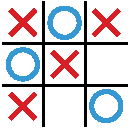
\includegraphics[width=0.15\textwidth]{figures/tic_env_win.pdf}
    } \hspace{0.2in}
    \subfloat[Win for \textsc{O}]{
        \label{fig:tic-env-loss}
        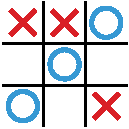
\includegraphics[width=0.15\textwidth]{figures/tic_env_loss.pdf}
    } \hspace{0.2in}
    \subfloat[Draw]{
        \label{fig:tic-env-draw}
        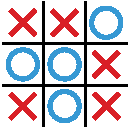
\includegraphics[width=0.15\textwidth]{figures/tic_env_draw.pdf}
    }
    \caption{Examples of wins, losses and draws in Tic-Tac-Toe}
    \label{fig:tic-env}
\end{figure}

As an example, we will simulate 10,000 games using a random players.

\begin{python}
from capstone.game import TicTacToe
game = TicTacToe()
game.legal_moves() # [1, 2, 3, 4, 5, 6, 7, 8, 9]
print(game)
\end{python}

%%%%%%%%%%%%%%%%%%%%%%%%%%%%%%%%%%%%%
\subsubsection{Connect 4 Environment}
%%%%%%%%%%%%%%%%%%%%%%%%%%%%%%%%%%%%%

\GithubURL{capstone/game/connect4.py}{Implementation}

Connect 4 is a two-player board game of perfect information where pieces are dropped into the
columns of a vertical $6 \times 7$ grid with the goal of forming a straight line of 4 connected
pieces. There are at most 7 actions per state, since placing a piece in a column is a legal action
only if that column has at least one empty location. \hyperref[fig:c4-env]{Figure~\ref*{fig:c4-env}}
shows three Connect 4 game positions.

%%%%%%%%%%
% Figure %
%%%%%%%%%%

\begin{figure}[!h]
    \centering
    \subfloat[Win for \textsc{Player 1}]{
        \label{fig:c4-env-wing}
        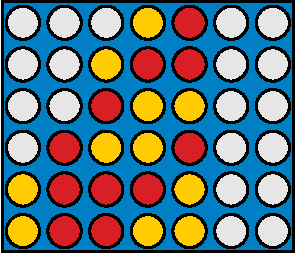
\includegraphics[width=0.2\textwidth]{figures/c4_env_win.pdf}
    } \hspace{0.1in}
    \subfloat[Win for \textsc{Player 2}]{
        \label{fig:c4-env-loss}
        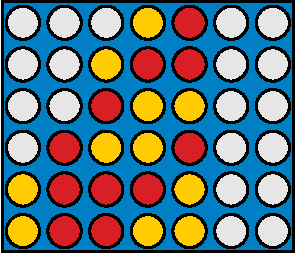
\includegraphics[width=0.2\textwidth]{figures/c4_env_loss.pdf}
    } \hspace{0.1in}
    \subfloat[Draw]{
        \label{fig:c4-env-draw}
        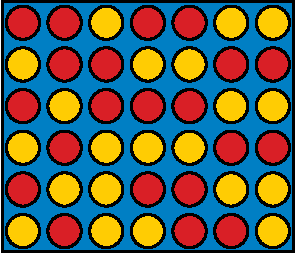
\includegraphics[width=0.2\textwidth]{figures/c4_env_draw.pdf}
    }
    \caption{Examples of wins, losses and draws in Connect Four}
    \label{fig:c4-env}
\end{figure}


%%%%%%%%%%%%%%%%%%%%%%%%%%%%%%%%%%%%%%
\subsubsection{UCI Connect 4 Data Set}
%%%%%%%%%%%%%%%%%%%%%%%%%%%%%%%%%%%%%%

\newcommand{\URLUCI}{\url{https://archive.ics.uci.edu/ml/datasets/Connect-4}}

As part of the testing phase, we will use the \emph{Connect 4 Data Set}\footnote{\URLUCI{}} that is
available from the UCI Machine Learning Repository~\citep{Hettich1998UCI}. This dataset has a total
of 67,557 instances, representing all legal 8-ply positions in \mbox{Connect 4} in which neither
player has won yet, and which the next move is not forced. Each instance is described by 42
features, one for each space in the $6 \times 7$ board, and can belong to one of the classes
$\{\textsc{x}, \textsc{o}, \textsc{b}\}$, where \textsc{x} is the first player, \textsc{o} is the
second player, and \textsc{b} is empty. The outcome class is the game theoretical value for the
first player, and can belong to one of the classes $\{\textsc{Win}, \textsc{Loss}, \textsc{Draw}\}$.
There are 44,473 wins, 16,635 losses and 6,449 draws.

%%%%%%%%%%%%%%%%%%%%%%%%%%%%%%%%%%%%%%
\subsection{Exploratory Visualization}
%%%%%%%%%%%%%%%%%%%%%%%%%%%%%%%%%%%%%%

%%%%%%%%%%%%%%%%%%%%%%%%%%%%%%%%%%%%%%
\subsubsection{UCI Connect 4 Data Set}
%%%%%%%%%%%%%%%%%%%%%%%%%%%%%%%%%%%%%%

As an example, here are ten instances selected randomly:

\definecolor{even}{RGB}{205,222,231}
\definecolor{odd}{RGB}{240,249,254}
\definecolor{header}{RGB}{128,169,188}
% \newcolumntype{R}{@{\extracolsep{13cm}}r@{\extracolsep{10pt}}}%

\begin{table}[h!]
\small
\centering
\renewcommand{\arraystretch}{1.2}
{\rowcolors{3}{even}{odd}
\begin{tabular}{ c | c c c c c c c c c c c c c c c c c | c }
\rowcolor{header}
 & \multicolumn{17}{c|}{\textbf{Features}} &  \textbf{Target} \\ \rowcolor{header}
\textbf{No.} & \textbf{a1} & \textbf{a2} & \textbf{a3} & \textbf{a4} & \textbf{a5} &
    \textbf{a6} & \textbf{b1} & \textbf{b2} & \textbf{...} & \textbf{f5} & \textbf{f6} &
    \textbf{g1} & \textbf{g2} & \textbf{g3} & \textbf{g4} & \textbf{g5} & \textbf{g6} & \textbf{outcome} \\ 
0      &  b &  b &  b &  b &  b &  b &  b &  b & ... &  b &  b &  b &  b &  b &  b &  b &  b &     win \\
1      &  b &  b &  b &  b &  b &  b &  b &  b & ... &  b &  b &  b &  b &  b &  b &  b &  b &     win \\
2      &  b &  b &  b &  b &  b &  b &  o &  b & ... &  b &  b &  b &  b &  b &  b &  b &  b &     win \\
3      &  b &  b &  b &  b &  b &  b &  b &  b & ... &  b &  b &  b &  b &  b &  b &  b &  b &     win \\
4      &  o &  b &  b &  b &  b &  b &  b &  b & ... &  b &  b &  b &  b &  b &  b &  b &  b &     win \\
...    & .. & .. & .. & .. & .. & .. & .. & .. & ... & .. & .. & .. & .. & .. & .. & .. & .. &     ... \\
67552  &  x &  x &  b &  b &  b &  b &  o &  x & ... &  b &  b &  o &  o &  x &  b &  b &  b &    loss \\
67553  &  x &  x &  b &  b &  b &  b &  o &  b & ... &  b &  b &  o &  x &  o &  o &  x &  b &    draw \\
67554  &  x &  x &  b &  b &  b &  b &  o &  o & ... &  b &  b &  o &  x &  x &  o &  b &  b &    loss \\
67555  &  x &  o &  b &  b &  b &  b &  o &  b & ... &  b &  b &  o &  x &  o &  x &  x &  b &    draw \\
67556  &  x &  o &  o &  o &  x &  b &  o &  b & ... &  b &  b &  x &  b &  b &  b &  b &  b &    draw \\
\end{tabular}
}
\caption{UCI Connect 4 Dataset. Each row represents a different board position, and each feature
         represents a specific cell in the board. The target is the outcome of the game for the
         first player, assuming perfect play.}
\label{table:uci-dataset}
\end{table}

\hyperref[fig:c4-exp]{Figure~\ref*{fig:c4-exp}} shows a visual representation of the 10 instances of
the data set.

%%%%%%%%%%
% Figure %
%%%%%%%%%%

\begin{figure}[!h]
    \centering
    \subfloat[Win]{
        \label{fig:c4-exp-1}
        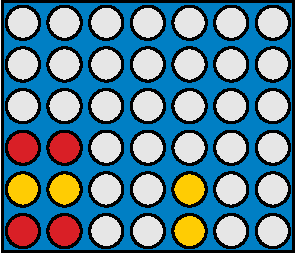
\includegraphics[width=0.15\textwidth]{figures/c4_exploration_1_win.pdf}
    } \hspace{0.1in}
    \subfloat[Loss]{
        \label{fig:c4-exp-2}
        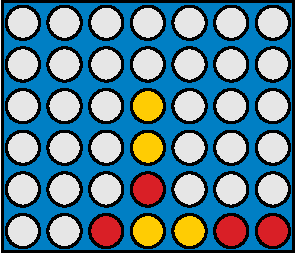
\includegraphics[width=0.15\textwidth]{figures/c4_exploration_2_loss.pdf}
    } \hspace{0.1in}
    \subfloat[Win]{
        \label{fig:c4-exp-3}
        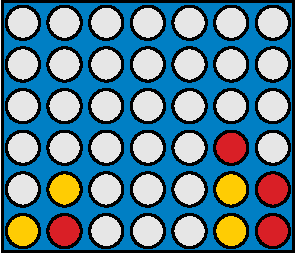
\includegraphics[width=0.15\textwidth]{figures/c4_exploration_3_win.pdf}
    } \hspace{0.1in}
    \subfloat[Loss]{
        \label{fig:c4-exp-4}
        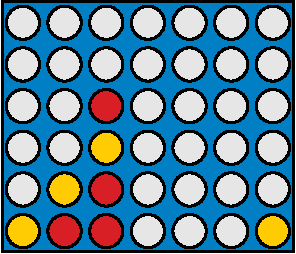
\includegraphics[width=0.15\textwidth]{figures/c4_exploration_4_loss.pdf}
    } \hspace{0.1in}
    \subfloat[Win]{
        \label{fig:c4-exp-5}
        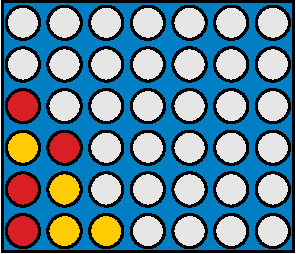
\includegraphics[width=0.15\textwidth]{figures/c4_exploration_5_win.pdf}
    } \hspace{0.1in}
    \subfloat[Draw]{
        \label{fig:c4-exp-6}
        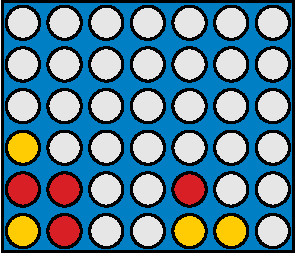
\includegraphics[width=0.15\textwidth]{figures/c4_exploration_6_draw.pdf}
    } \hspace{0.1in}
    \subfloat[Win]{
        \label{fig:c4-exp-7}
        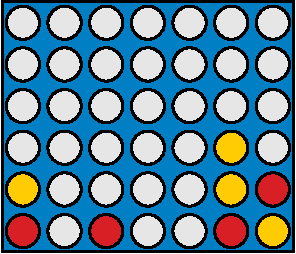
\includegraphics[width=0.15\textwidth]{figures/c4_exploration_7_win.pdf}
    } \hspace{0.1in}
    \subfloat[Win]{
        \label{fig:c4-exp-8}
        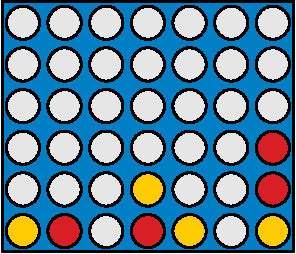
\includegraphics[width=0.15\textwidth]{figures/c4_exploration_8_win.pdf}
    } \hspace{0.1in}
    \subfloat[Loss]{
        \label{fig:c4-exp-9}
        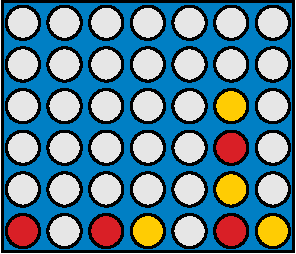
\includegraphics[width=0.15\textwidth]{figures/c4_exploration_9_loss.pdf}
    } \hspace{0.1in}
    \subfloat[Draw]{
        \label{fig:c4-exp-10}
        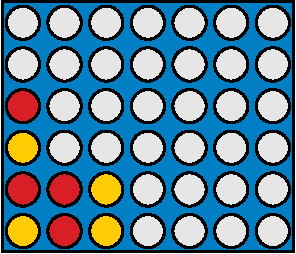
\includegraphics[width=0.15\textwidth]{figures/c4_exploration_10_draw.pdf}
    }
    \caption{10 randomly selected instances of the UCI Connect 4 Data Set. The outcome of each board
    position is from the point of view of the firs player (Yellow discs).}
    \label{fig:c4-exp}
\end{figure}

%%%%%%%%%%%%%%%%%%%%%%%%%%%%%%%%%%%%%%
\subsection{Algorithms and Techniques}
%%%%%%%%%%%%%%%%%%%%%%%%%%%%%%%%%%%%%%

%%%%%%%%%%%%%%%%%%%%%%%%%%%%%%%%%%
\subsubsection{Alpha-beta pruning}
%%%%%%%%%%%%%%%%%%%%%%%%%%%%%%%%%%

\GithubURL{capstone/player/alphabeta.py}{Implementation}

% In this project, we will use reinforcement learning with deep learning to make an agent learn to
% play the game of {Connect 4}\footnote{\url{\URLcf}} by playing games against itself. In other words,
% using the formalism used by \cite{Mitchell1997Book} to define a machine learning problem:

\emph{Alpha-beta pruning}~\citep{Knuth1975AB} is the most common game tree search algorithm for
two-player games of perfect information. It extends the minimax algorithm to reduce the number of
nodes that are evaluated in the game tree. Instead of calculating the exact minimax values for all
the nodes in the game tree, alpha-beta prunes away branches that will not have any effect in the
selection of the best move.

% \hyperref[fig:ab-game-tree]{Figure~\ref*{fig:ab-game-tree}} illustrates
% the prunning process in the Alpha-Beta algorithm. This tree has a total of 28 nodes, however, 10
% nodes of the tree were pruned (crossed branches) because those branches do not have any effect in
% the selection of the best move.

% The algorithm works by imposing a \emph{search window} $\left[ \alpha, \beta \right] $ at each
% \textsc{Min} or \textsc{Max} node in the game tree. $\alpha$ represents the value of the best (i.e.
% highest-value) node found so far for \textsc{Max}, while $\beta$ is the best value (i.e.
% lowest-value) for \textsc{Min}. The search through successor nodes can be terminated as soon as the
% current node's value is proven to fall outside the search window. The functionality of Alpha-Beta
% is detailed in \hyperref[alg:alpha-beta]{Algorithm~\ref*{alg:alpha-beta}}.

% \newcommand{\URLab}{https://github.com/davidrobles/mlnd-capstone-code/blob/master/capstone/player/alphabeta.py}

%%%%%%%%%%%%%%%%%%%%%%%%%%
\subsubsection{Q-learning}
%%%%%%%%%%%%%%%%%%%%%%%%%%

\GithubURL{capstone/algorithms/qlearning.py}{Implementation}

One of the most basic and popular methods to estimate action-value functions is the
\emph{Q-learning} algorithm~\citep{Watkins1989PhD}. It is model-free online off-policy algorithm,
whose main strength is that it is able to compare the expected utility of the available actions
without requiring a model of the environment. Q-learning works by learning an action-value function
that gives the expected utility of taking a given action in a given state and following a fixed
policy thereafter. The update rule uses action-values and a built-in max-operator over the
action-values of the next state in order to update $Q(s_t, a_t)$ as follows,
%
\begin{equation}
    Q(s_t, a_t) \gets Q(s_t, a_t) + \alpha [r_{t+1} + \gamma \max_a Q(s_{t+1}, a) - Q(s_t, a_t)]
\end{equation}

The agent makes a step in the environment from state $s_t$ to $s_{t+1}$ using action $a_t$ while
receiving reward $r_t$. The update takes place on the action-value $a_t$ in the state $s_t$ from
which this action was executed.

Q-learning is exploration-intensive, which means that it will converge to the optimal policy
regardless of the exploration policy being followed, under the assumption that each state-action
pair is visited an infinite number of times, and the learning parameter $\alpha$ is decreased
appropriately~\citep{Watkins1992Q}.

\subsubsection{Self-play}

Self-play is by far the most popular training method. It is a single policy $\pi(s,a)$ that is used
by both players in a two-player game, $\pi_1(s,a) = \pi_2(s,a) = \pi(s,a)$. The first reason for its
popularity is that training is quickest if the learner's opponent is roughly equally strong, and
that definitely holds for self-play. As a second reason for popularity, there is no need to
implement or access a different agent with roughly equal playing strength. However, self-play has
several drawbacks, with the main one being that a single opponent does not provide sufficient
exploration~\citep{Szita2011RLGames}.

%%%%%%%%%%%%%%%%%%%%%%
\subsection{Benchmark}
\label{sec:benchmark}
%%%%%%%%%%%%%%%%%%%%%%

\begin{itemize}

    \item \textbf{Random agent}. This benchmark consists in playing against an agent that takes
        uniformly random moves. This is the most basic benchmark, but first we have to be sure that
        our learned evaluation function can play better than a random agent before moving into a
        harder benchmark. Also, this will help us to detect bugs in the code and algorithms: if a
        learned value function does not play significantly better than a random agent, is not
        learning. The idea is to test against this benchmark using Alpha-beta pruning at 1, 2 and
        4-ply search.

    \item \textbf{Connect 4 Data Set}. This dataset will be used as the main benchmark. The learned
        value function will be used to predict the game-theoretic outcomes (win, loss or draw) for
        the first player in the 67,557 instances of the dataset.

\end{itemize}

%%%%%%%%%%%%%%%%%%%%%%%%%%%%%%%%%%%%%%%%%%%%%%%%%%%%%%%%%%%%%%%%%%%%%%%%%%%%%%%%%%%%%%%%%%%%%%%%%%%%
\section{Implementation}
%%%%%%%%%%%%%%%%%%%%%%%%%%%%%%%%%%%%%%%%%%%%%%%%%%%%%%%%%%%%%%%%%%%%%%%%%%%%%%%%%%%%%%%%%%%%%%%%%%%%

%%%%%%%%%%%%%%%%%%%%%%%%%%%%%%%%%%%%
\subsection{Markov Decision Process}
%%%%%%%%%%%%%%%%%%%%%%%%%%%%%%%%%%%%

\GithubURL{capstone/mdp/mdp.py}{Implementation}

A \emph{Markov decision process} (MDP) consist of a set of states, a set of actions, a transition
function and a reward function.

\begin{itemize}

    \item $\mathcal{S}$ is the set of \emph{states} (state space).

    \item $\mathcal{A}$ is the set of \emph{actions} (action space). The set of actions that are
      available in some particular state $s_t \in \mathcal{S}$ is denoted $\mathcal{A}(s_t)$, such
      that $\mathcal{A}(s_t) \in \mathcal{P}(\mathcal{A})$, where $\mathcal{P}(\cdot)$ denotes the
      power set.

    \item $ T : \mathcal{S} \times \mathcal{A} \times \mathcal{S} \to \mathbb{R}$ is the
      \emph{transition function}, which is the probability given we are in state $s_t \in
      \mathcal{S}$, take action $a_t \in \mathcal{A}(s_t)$ and we will transition to state $s_{t+1}
      \in \mathcal{S}$.

    \item $ R : \mathcal{S} \times \mathcal{A} \times \mathcal{S} \to \mathbb{R}$ is the
      \emph{reward function}, which is the immediate reward received when in state $s_t \in
      \mathcal{S}$ action $a_t \in \mathcal{A}$ is taken and the MDP transitions to state $s_{t+1}
      \in \mathcal{S}$. However, it is also possible to define it either as $ R : \mathcal{S} \times
      \mathcal{A} \to \mathbb{R}$ or $R : \mathcal{S} \to \mathbb{R}$. The first one gives rewards
      for performing an action $a_t$ in a particular state $s_t$, and the second gives rewards when
      transitioning to state $s_{t+1}$.

\end{itemize}

%%%%%%%%%%%%%%%%%%%%%%%%
\subsection{Environment}
%%%%%%%%%%%%%%%%%%%%%%%%

\GithubURL{capstone/environment/environment.py}{Implementation}

An agent does not have access to the dynamics (reward and transition function) of the MDP. However,
it interacts with an \emph{environment} by way of three signals: a \emph{state}, which describes the
state of the environment, an \emph{action}, which allows the agent to have some impact on the
environment, and a \emph{reward}, which provides the agent with feedback on its immediate
performance.

%%%%%%%%%%%%%%%%%%%
\subsection{Policy}
%%%%%%%%%%%%%%%%%%%

\GithubURL{capstone/policy/policy.py}{Implementation}

In an MDP, the agent acts according to a policy $\pi$, which maps each state $s \in \mathcal{S}$ to
an action $a \in \mathcal{A}(s)$. A policy that specifies a unique action to be performed is called
a \emph{deterministic} policy, and is defined as $\pi : \mathcal{S} \rightarrow \mathcal{A}$. On the
other hand, a \emph{stochastic} policy $\pi : \mathcal{S} \times \mathcal{A} \rightarrow [0,1]$
selects actions according to a probability distribution, such that for each state $s \in
\mathcal{S}$, it holds that $\pi(s,a) \geq 0$ and $\sum_{a\in\mathcal{A}(s)} \pi(s,a) = 1$.

The interaction between the policy used by the agent and the environment works as follows. First, it
starts at an \emph{initial state} $s_0$. Then, the policy $\pi$ selects an action $a_0 = \pi(s_0)$
from the set of available actions $\mathcal{A}(s_0)$, and the action is executed. The environment
transitions to a new state $s_1$ based on the transition function $T$ with probability
$T(s_0,a_0,s_1)$, and a reward $r_0 = R(s_0, a_0, s_1)$ is received. This process continues,
producing a \emph{trajectory} of experience $s_0, a_0, s_1, r_1, a_1, s_2, r_2, a_2, \dots$. If the
task is \emph{episodic}, the process ends in a \emph{terminal state} $s_T$ and is restarted in the
initial state. If the task is \emph{continiuing}, the sequence of states can be extended
indefinitely.

%%%%%%%%%%%%%%%%%%%%%%%%%%%%%
\subsubsection{Random policy}
%%%%%%%%%%%%%%%%%%%%%%%%%%%%%

\GithubURL{capstone/policy/random_policy.py}{Implementation}

Selects:
%
\begin{equation}
    \pi_{\textrm{rand}}(s) = \argmax_{a \in \mathcal{A}(s_t)} Q(s, a)
\end{equation}

%%%%%%%%%%%%%%%%%%%%%%%%%%%%%
\subsubsection{Greedy policy}
%%%%%%%%%%%%%%%%%%%%%%%%%%%%%

\GithubURL{capstone/policy/greedy.py}{Implementation}

\noindent
\href{https://github.com/davidrobles/mlnd-capstone-code/blob/master/capstone/policy/greedy.py}
     {Implementation}
\break

The greedy tree policy selects the \emph{max action}, which is the greedy action with the highest
value.
%
\begin{equation}
    \pi_{\textrm{greedy}}(s) = \argmax_{a \in \mathcal{A}(s_t)} Q(s, a)
\end{equation}

%%%%%%%%%%%%%%%%%%%%%%%%%%%%%%%%%
\subsubsection{$\epsilon$-greedy}
%%%%%%%%%%%%%%%%%%%%%%%%%%%%%%%%%

\GithubURL{capstone/policy/egreedy.py}{Implementation}

The $\epsilon$-greedy tree policy selects the best action for a proportion $1 - \epsilon$ of the
trials, and another action is randomly selected (with uniform probability) for a proportion
$\epsilon$,
%
\begin{equation}
    \pi_{\epsilon}(s) = \left\{
     \begin{array}{lr}
         \pi_{\textrm{rand}}(s,a) & \text{if } rand() < \epsilon\\
         \pi_{\textrm{greedy}}(s,a) & \text{otherwise}
     \end{array}
   \right.
\end{equation}
%
where $\epsilon \in [0, 1]$ and $rand()$ returns a random number from a uniform distribution $\in
[0, 1]$.

%%%%%%%%%%%%%%%%%
\subsection{Game}
%%%%%%%%%%%%%%%%%

Informally speaking, a perfect-information game in extensive form is a tree in the sense of graph
theory, in which each node represents the current state of the game, each edge represents a
possible action, and the leaves represent the terminal states, which contains final outcomes
through a utility function. In the field of AI these are known simply as \emph{game trees}.

A \textbf{perfect-information extensive-form game} is defined as a tuple $G = (n, \mathcal{S},
\mathcal{S_T}, \mathcal{A}, \rho, T, U)$, where:


\begin{itemize}

    \item $n$ is the \emph{number of players};

    \item $\mathcal{S}$ is the set of \emph{states};

    \item $\mathcal{S}_T \subset \mathcal{S}$ is the set of \emph{terminal states};

    \item $\mathcal{A}$ is the set of \emph{actions}. The set of actions that are available in some
    particular state $s_t \in \mathcal{S}$ for the player in turn $\rho(s_t)$ is denoted
    $\mathcal{A}(s_t)$, such that $\mathcal{A}(s_t) \in \mathcal{P}(\mathcal{A})$, where
    $\mathcal{P}(\cdot)$ denotes the power set.

    \item $\rho : \overline{\mathcal{S}_T} \to \{i \in \mathbb{N} : 1 \leq i \leq n \} $ is the
    \emph{player function}, which assigns to each non-terminal state $s_t \in \overline{S_T}$ a
    player $i$ who chooses an action at that state;

    \item $T : \overline{\mathcal{S}_T} \times \mathcal{A} \to \mathcal{S}$ is the \emph{transition
    function}, which maps a non-terminal state and an action to a new state;

    \item $U : S_T \to \mathbb{R}^n $ is the \emph{utility function}, which returns a vector of
    payoffs $U(s_T) = (u_1, \dots, u_n)$ for each of the $n$ players of the game. We will use the
    notation $U_i(s_T)$ to represent the payoff for the $i$th player when the game is over at state
    $s_T \in S_T$.

\end{itemize}

In two-player perfect-information extensive-form games, a \emph{ply} refers to one turn taken by one
of the players.

%%%%%%%%%%%%%%%%%%%%%%%%%%%%%%%%%%%%%%%%%%%%%%%%%%%%%%%%%%%%%%%%%%%%%%%%%%%%%%%%%%%%%%%%%%%%%%%%%%%%
\section{Methodology}
%%%%%%%%%%%%%%%%%%%%%%%%%%%%%%%%%%%%%%%%%%%%%%%%%%%%%%%%%%%%%%%%%%%%%%%%%%%%%%%%%%%%%%%%%%%%%%%%%%%%

%%%%%%%%%%%%%%%%%%%%%%%%%%%%%%%
\subsection{Data Preprocessing}
%%%%%%%%%%%%%%%%%%%%%%%%%%%%%%%

Content.

%%%%%%%%%%%%%%%%%%%%%%%%%%%
\subsection{Implementation}
%%%%%%%%%%%%%%%%%%%%%%%%%%%

\begin{itemize}

    \item Two games were implemented: Tic Tac Toe and Connect 4.
    \item Converting a to an MDP by using a fixed agent.
    \item Show that q-learning learns to play against a fixed opponent using Tic-Tac-Toe.
    \item Show that q-learning learns to play against a fixed opponent using Connect 4.

\end{itemize}

%%%%%%%%%%%%%%%%%%%%%%%
\subsection{Refinement}
%%%%%%%%%%%%%%%%%%%%%%%

Content.

%%%%%%%%%%%%%%%%%%
\subsection{Games}
%%%%%%%%%%%%%%%%%%

%%%%%%%%%%%%%%%%%%%%%%%%%%%
\subsubsection{Tic Tac Toe}
%%%%%%%%%%%%%%%%%%%%%%%%%%%

\GithubURL{capstone/game/tictactoe.py}{Implementation}



\subsubsection{GameMDP converter}

Converting an MDP

%%%%%%%%%%%%%%%%%%%%%%%%%%%%%%%%%%%%%%%%%%%%%%%%%%%%%%%%%%%%%%%%%%%%
\section{Examples}
%%%%%%%%%%%%%%%%%%%%%%%%%%%%%%%%%%%%%%%%%%%%%%%%%%%%%%%%%%%%%%%%%%%%

%%%%%%%%%%%%%%%%%%%%%%%%%%%%%%%%%%%%%%%%%%%%%%%%%%%%%%%%%%%%%%%%%%
\subsection{Estimate state-action values using tabular Q-learning}
%%%%%%%%%%%%%%%%%%%%%%%%%%%%%%%%%%%%%%%%%%%%%%%%%%%%%%%%%%%%%%%%%%

In this example we will estimate the state-action values for two very simple board positions for
both Tic-Tac-Toe and Connect 4. We will be using the tabular version of Q-learning. The goal here is
simply to verify that our implementation of the Q-learning algorithm is working as expected. We
chose very simple positions because the expected q-values are easy to understand.

We converted both games as MDPs by making the opponent a fixed agent that takes optimal moves by
using the Alpha-Beta algorithm. This allowed us to verify that we are learning the q-values assuming
the worst case scenario. In other situations in which the depth of the game tree is huge Alpha-Beta
would need to combined with a good heuristic evaluation function, but in these simple positions it
won't be necessary.

The rewards given by the Tic-Tac-Toe environment are $+1$ for a win for the first player, $-1$ for a
win for the first player, and $0$ for a draw.

%%%%%%%%%%%%%%%%%%%%%%%%%%%
\subsubsection{Tic-Tac-toe}
%%%%%%%%%%%%%%%%%%%%%%%%%%%

% - Implement Q-learning
% - GameMDP converter
% - Generate a Tic-Tac-Toe board that is easier to analyze
% - Run Q-learning and show that the values are correct.

% \GithubURL{examples/tic_ql_tabular_fixed.py}{Implementation}

For Tic-Tac-Toe we used the board position in \hyperref[fig:tic-ql-tab-cur]
{Figure~\ref*{fig:tic-ql-tab-cur}} as the starting state, $s_0$. It has five available actions,
$\mathcal{A}(s_0) = \{1, 2, 4, 6, 9\}$. By looking at such a simple position we can clearly identify
that the best available action is 9, which leads to a win if we keep playing the best possible
actions. Any other action (i.e. 1, 2, 4 or 6) would lead to a loss, assuming perfect play from the
opponent.

\begin{figure}[!h]
    \centering
    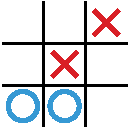
\includegraphics[width=0.15\textwidth]{figures/tic_ql_tab_current.pdf}
    \caption{Starting Tic-Tac-Toe state, $s_0$, with five legal actions, $\mathcal{A}(s_0) = \{1, 2, 4, 6, 9\}$.}
    \label{fig:tic-ql-tab-cur}
\end{figure}

We ran the tabular version of the Q-learning algorithm with $\alpha = 0.1$ (learning rate),
$\gamma=1.0$ (discount factor), and a uniformly random behavior policy. The Q-values converged to
the expected values after around 800 episodes of training, and are shown in
\hyperref[fig:tic-ql-qvalues] {Figure~\ref*{fig:tic-ql-qvalues}}. As we can see in
\hyperref[fig:tic-ql-tab-move-9] {Figure~\ref*{fig:tic-ql-tab-move-9}}, the expected future reward
of taking action 9 is correctly estimated as 1.0, since that would lead to a win. At the same time,
the q-values for all the other actions was -1.0. This makes sense, since any action not being 9
would lead to an immediate loss. Also, we can see in \hyperref[fig:tic-ql-tab-qvalues-progress]
{Figure~\ref*{fig:tic-ql-tab-qvalues-progress}} we can see the predicted q-values for each available
action. It is interesting to see how the q-value for $Q(s_0, 9)$ takes some time to converge. This
is probably because taking action 9 leads to an eventual win, but not immediately. It requires
making another move (either 1 or 6) to win.

% show the index numbers of the board

%%%%%%%%%%
% Figure %
%%%%%%%%%%

\begin{figure}[!h]
    \centering
    \subfloat[$Q(s_0, 1) = -1.0$]{
        \label{fig:tic-ql-tab-move-1}
        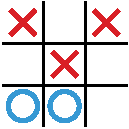
\includegraphics[width=0.15\textwidth]{figures/tic_ql_tab_move_1.pdf}
    } \hspace{0.1in}
    \subfloat[$Q(s_0, 2) = -1.0$]{
        \label{fig:tic-ql-tab-move-2}
        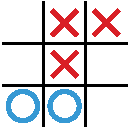
\includegraphics[width=0.15\textwidth]{figures/tic_ql_tab_move_2.pdf}
    } \hspace{0.1in}
    \subfloat[$Q(s_0, 4) = -1.0$]{
        \label{fig:tic-ql-tab-move-4}
        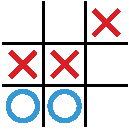
\includegraphics[width=0.15\textwidth]{figures/tic_ql_tab_move_4.pdf}
    } \hspace{0.1in}
    \subfloat[$Q(s_0, 6) = -1.0$]{
        \label{fig:tic-ql-tab-move-6}
        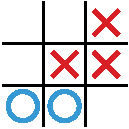
\includegraphics[width=0.15\textwidth]{figures/tic_ql_tab_move_6.pdf}
    } \hspace{0.1in}
    \subfloat[$Q(s_0, 9) = 1.0$]{
        \label{fig:tic-ql-tab-move-9}
        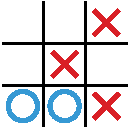
\includegraphics[width=0.15\textwidth]{figures/tic_ql_tab_move_9.pdf}
    }
    \caption{}
    \label{fig:tic-ql-qvalues}
\end{figure}

%%%%%%%%%%
% Figure %
%%%%%%%%%%

\begin{figure}[!h]
    \centering
    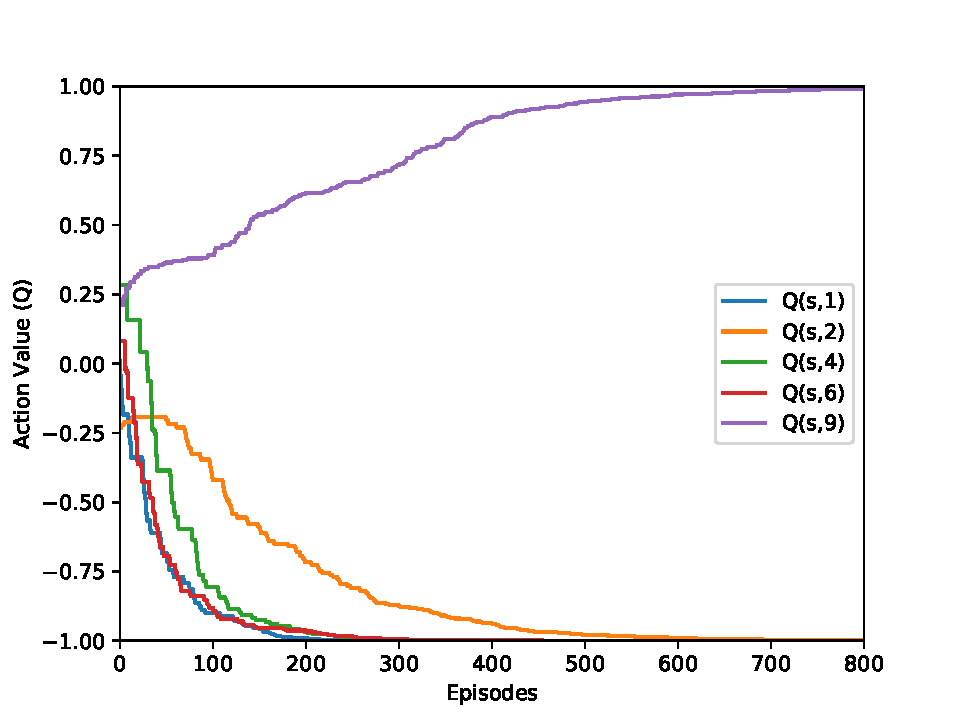
\includegraphics[width=0.40\textwidth]{figures/tic_ql_tab_action_values.pdf}
    \caption{The predicted state-action value during training.}
    \label{fig:tic-ql-tab-qvalues-progress}
\end{figure}

%%%%%%%%%%%%%%%%%%%%%%%%%
\subsubsection{Connect 4}
%%%%%%%%%%%%%%%%%%%%%%%%%

%%% MERGE THIS WITH PREVIOSU CHAPTER< SUBFIGURES

% \GithubURL{examples/c4_ql_tabular_fixed.py}{Implementation}

For Connect 4 we used the board position in \hyperref[fig:c4-ql-tab-cur]
{Figure~\ref*{fig:c4-ql-tab-cur}} as the starting state, $s_0$. It has three available actions,
$\mathcal{A}(s_0) = \{\texttt{d}, \texttt{f}, \texttt{g}\}$. By looking at such a simple position we
can clearly identify that the best available action is \texttt{f}, which leads to a win if we keep
playing the best possible actions.  Any other action (i.e. \texttt{d} or \texttt{g}) would lead to a
loss, assuming perfect play from the opponent.

%%%%%%%%%%
% Figure %
%%%%%%%%%%

\begin{figure}[!h]
    \centering
    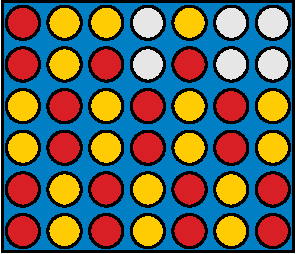
\includegraphics[width=0.2\textwidth]{figures/c4_ql_tab_current.pdf}
    \caption{Connect 4 board, $s_0$, with three legal actions: $\{\texttt{d}, \texttt{f}, \texttt{g}\}$.}
    \label{fig:c4-ql-tab-cur}
\end{figure}

We ran the same tabular version of the Q-learning algorithm with the same parameters as the used for
Tic-Tac-Toe $\alpha=0.1$ (learning rate), $\gamma=1.0$ (discount factor), and a uniformly random
behavior policy. The Q-values also converged to the expected values after around 800 episodes of
training, and are shown in \hyperref[fig:c4-ql-qvalues] {Figure~\ref*{fig:c4-ql-qvalues}}. As we can
see in \hyperref[fig:c4-ql-move-f] {Figure~\ref*{fig:c4-ql-move-f}}, the expected future reward of
taking action \texttt{f} is correctly estimated as 1.0, since that would lead to a win. At the same
time, the q-values for all the other actions was -1.0. This makes sense, since any action not being
\texttt{f} would lead to an immediate loss. Also, we can see in
\hyperref[fig:c4-ql-tab-qvalues-progress] {Figure~\ref*{fig:c4-ql-tab-qvalues-progress}} we can see
the predicted q-values for each available action. 

%%%%%%%%%%%
% Figures %
%%%%%%%%%%%

\begin{figure}[!b]
    \centering
    \subfloat[$Q(s_0, \texttt{d}) = -1.0$]{
        \label{fig:c4-ql-move-e}
        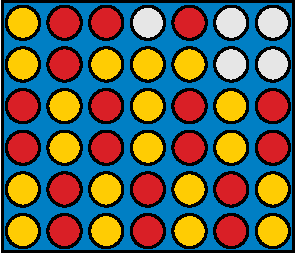
\includegraphics[width=0.2\textwidth]{figures/c4_ql_tab_move_d.pdf}
    } \hspace{0.1in}
    \subfloat[$Q(s_0, \texttt{f}) = 1.0$]{
        \label{fig:c4-ql-move-f}
        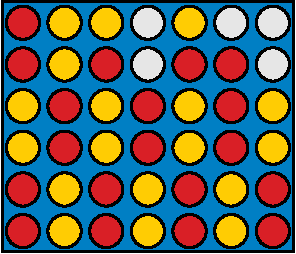
\includegraphics[width=0.2\textwidth]{figures/c4_ql_tab_move_f.pdf}
    } \hspace{0.1in}0
    \subfloat[$Q(s_0, \texttt{g}) = -1.0$]{
        \label{fig:c4-ql-move-g}
        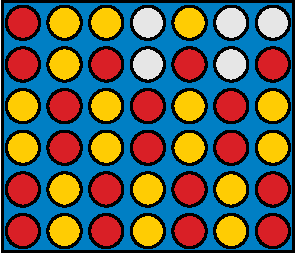
\includegraphics[width=0.2\textwidth]{figures/c4_ql_tab_move_g.pdf}
    }
    \caption{All the next states and their q values.}
    \label{fig:c4-ql-qvalues}
\end{figure}

%%%%%%%%%%
% Figure %
%%%%%%%%%%

\begin{figure}[!h]
    \centering
    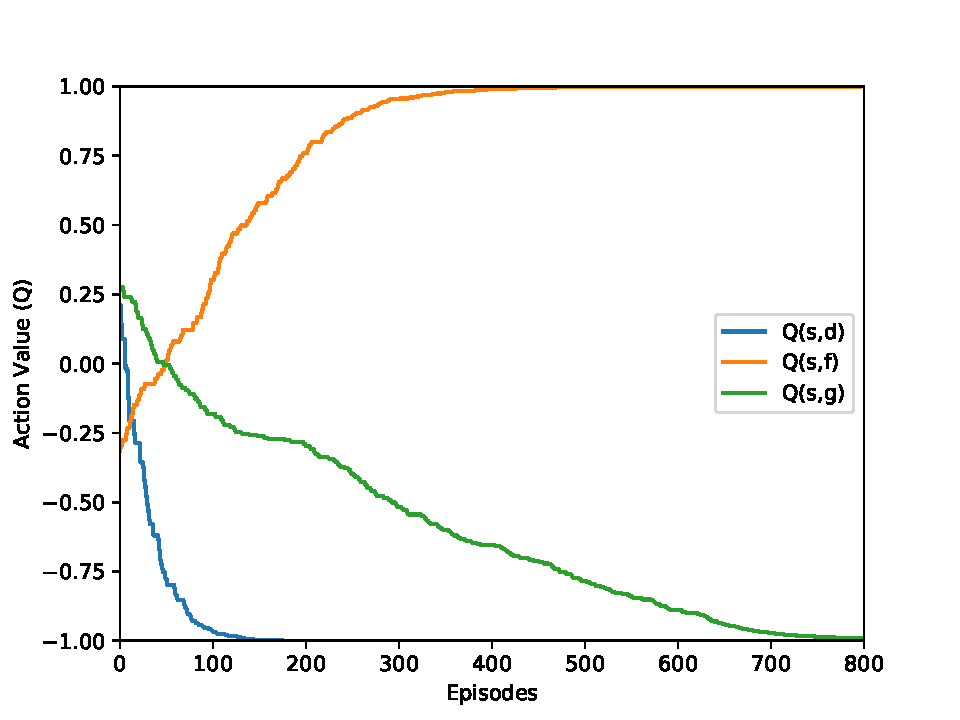
\includegraphics[width=0.50\textwidth]{figures/c4_ql_tab_action_values.pdf}
    \caption{The predicted state-action value during training.}
    \label{fig:c4-ql-tab-qvalues-progress}
\end{figure}

%%%%%%%%%%%%%%%%%%%%%%%%%%%%%%%%%%%%%%%%%%%%%%%%%%%%%%%%%%%%%
\subsection{Estimate q-values using Q-learning via self-play}
%%%%%%%%%%%%%%%%%%%%%%%%%%%%%%%%%%%%%%%%%%%%%%%%%%%%%%%%%%%%%

In the previous example we estimated the q-values for Tic-Tac-toe and Connect 4 positions against a
fixed Alpha-Beta opponent. While this works very well sometimes we don't have that algorithm. An
alternative is to use self-play, which consists in making playing games against itself.

% examples/tic_ql_tab_simple_selfplay.py 

%%%%%%%%%%%
% Figures %
%%%%%%%%%%%

\begin{figure}[!h]
    \centering
    \subfloat[Tic-Tac-Toe]{
        \label{fig:tic-ql-tab-simple-selfplay-progress}
        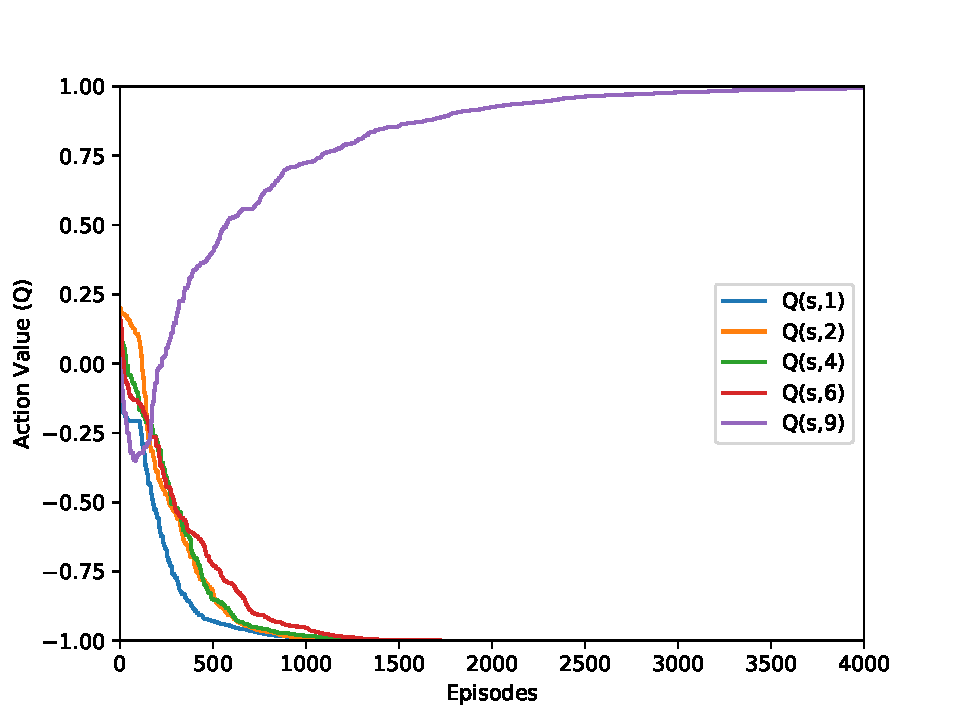
\includegraphics[width=0.4\textwidth]{figures/tic_ql_tab_simple_selfplay_progress.pdf}
    } \hspace{0.1in}
    \subfloat[Connect 4]{
        \label{fig:c4-ql-tab-simple-selfplay-progress}
        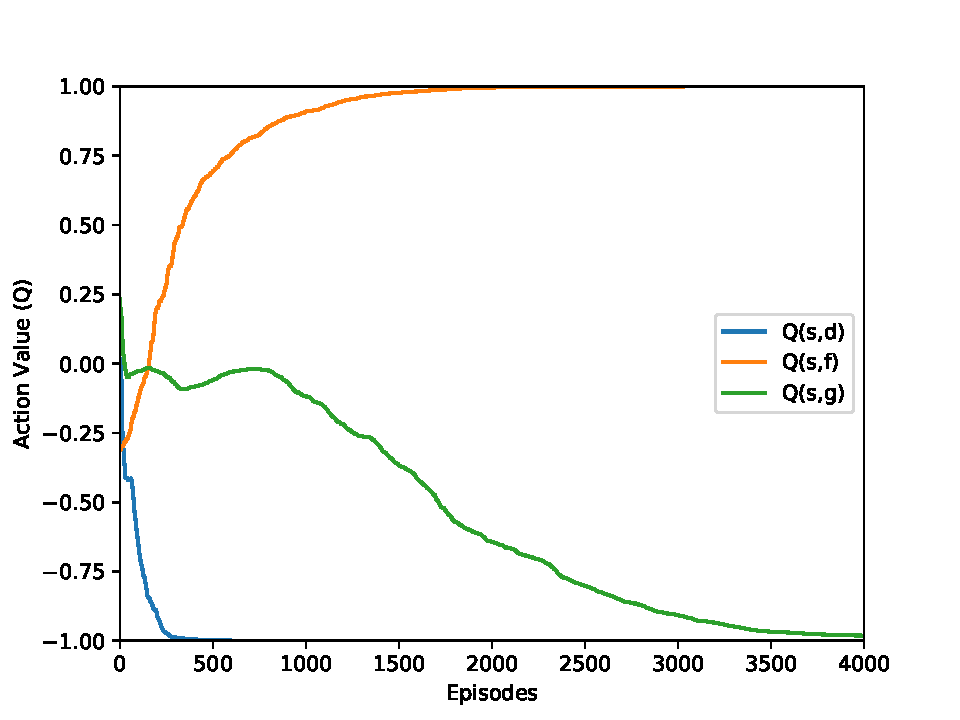
\includegraphics[width=0.4\textwidth]{figures/c4_ql_tab_simple_selfplay_progress.pdf}
    }
    \caption{All the next states and their q values.}
    \label{fig:ql-tab-simple-selfplay-progress}
\end{figure}

% This converged to examples/tic_ql_tab_simple_selfplay.py

In both examples we can see that it took longer to learn the episodes because it didn't have a
perfect guidance on what was good and bad, it had to learn it by itself. This is a powerful
technique that will be used in the next sections to learn a value function for Connect 4. The values
are the same as the ones shown in Figures \hyperref[fig:tic-ql-qvalues]{\ref*{fig:tic-ql-qvalues}}
and \hyperref[fig:c4-ql-qvalues]{\ref*{fig:c4-ql-qvalues}}.

%%%%%%%%%%%%%%%%%%%%%%%%%%%%%%%%%%%%%%%%%%%%%%%%%%%%%%%%%%%
\subsection{Estimate all q-values using tabular Q-learning}
%%%%%%%%%%%%%%%%%%%%%%%%%%%%%%%%%%%%%%%%%%%%%%%%%%%%%%%%%%%

% examples/tic_ql_tab_full_fixed.py

Now the idea is to learn to play the games in general starting from the same position. This means
that we will use Q-learning to estimate the q-values from the empty board of the game. We will do it
for Tic-Tac-Toe. We ran the experiment using similar parameters, and after 65,000 episodes the
q-values were found correctly.

% IDEA, Juntar ambos tic tac toe and connect 4 en uno!

In \hyperref[fig:tic-ql-tab-full-wld-plot]{Figure~\ref*{fig:tic-ql-tab-full-wld-plot}} we can see
how after 65,000 episodes it learned the values.

%%%%%%%%%%
% Figure %
%%%%%%%%%%

\begin{figure}[!h]
    \centering
    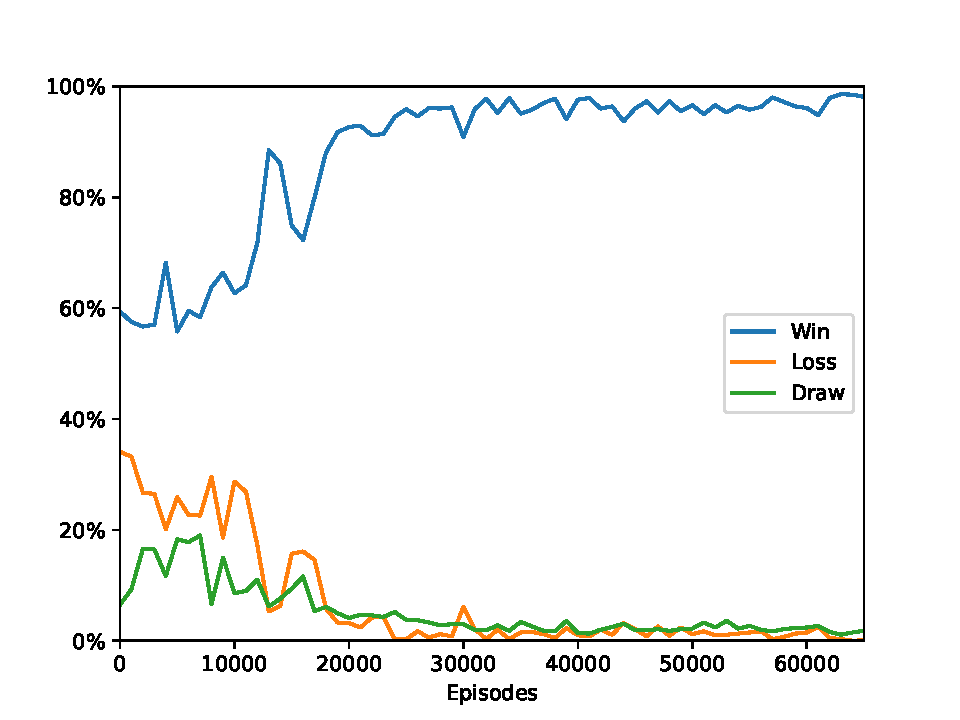
\includegraphics[width=0.50\textwidth]{figures/tic_ql_tab_full_wld_plot.pdf}
    \caption{Results after playing 1,000 games every 1,000 episodes against a Random player.}
    \label{fig:tic-ql-tab-full-wld-plot}
\end{figure}

%%%%%%%%%%%%%%%%%%%%%%%%%%%%%%%%%%%%%%%%%%%%%%%%%%%%%%%%%%%%%%%%%%%%%%%%%%%%%%%%%%%%%%%%%%%%%%%%%%%%
\section{Results}
%%%%%%%%%%%%%%%%%%%%%%%%%%%%%%%%%%%%%%%%%%%%%%%%%%%%%%%%%%%%%%%%%%%%%%%%%%%%%%%%%%%%%%%%%%%%%%%%%%%%

%%%%%%%%%%%%%%%%%%%%%%%%%%%%%%%%%%%%%%%%%%%%
\subsection{Model Evaluation and Validation}
%%%%%%%%%%%%%%%%%%%%%%%%%%%%%%%%%%%%%%%%%%%%

Content.

%%%%%%%%%%%%%%%%%%%%%%%%%%
\subsection{Justification}
%%%%%%%%%%%%%%%%%%%%%%%%%%

Content.

%%%%%%%%%%%%%%%%%%%%%%%%%%%%%%%%%%%%%%%%%%%%%%%%%%%%%%%%%%%%%%%%%%%%%%%%%%%%%%%%%%%%%%%%%%%%%%%%%%%%
\section{Conclusion}
%%%%%%%%%%%%%%%%%%%%%%%%%%%%%%%%%%%%%%%%%%%%%%%%%%%%%%%%%%%%%%%%%%%%%%%%%%%%%%%%%%%%%%%%%%%%%%%%%%%%

%%%%%%%%%%%%%%%%%%%%%%%%%%%%%%%%%%%%
\subsection{Free-Form Visualization}
%%%%%%%%%%%%%%%%%%%%%%%%%%%%%%%%%%%%

Content.

%%%%%%%%%%%%%%%%%%%%%%%
\subsection{Reflection}
%%%%%%%%%%%%%%%%%%%%%%%

Content.

%%%%%%%%%%%%%%%%%%%%%%%%
\subsection{Improvement}
%%%%%%%%%%%%%%%%%%%%%%%%

Content.

%%%%%%%%%%%%%%%%%%%%%%%%%%%%%%%%%%%%%%%%%%%%%%%%%%%%%%%%%%%%%%%%%%%%%%%%%%%%%%%%%%%%%%%%%%%%%%%%%%%%
% BIBLIOGRAPHY
%%%%%%%%%%%%%%%%%%%%%%%%%%%%%%%%%%%%%%%%%%%%%%%%%%%%%%%%%%%%%%%%%%%%%%%%%%%%%%%%%%%%%%%%%%%%%%%%%%%%

\bibliographystyle{plainnat}
\bibliography{bibliography}

\end{document}
